\begin{center}
    \begin{figure}[H]
        \centering

        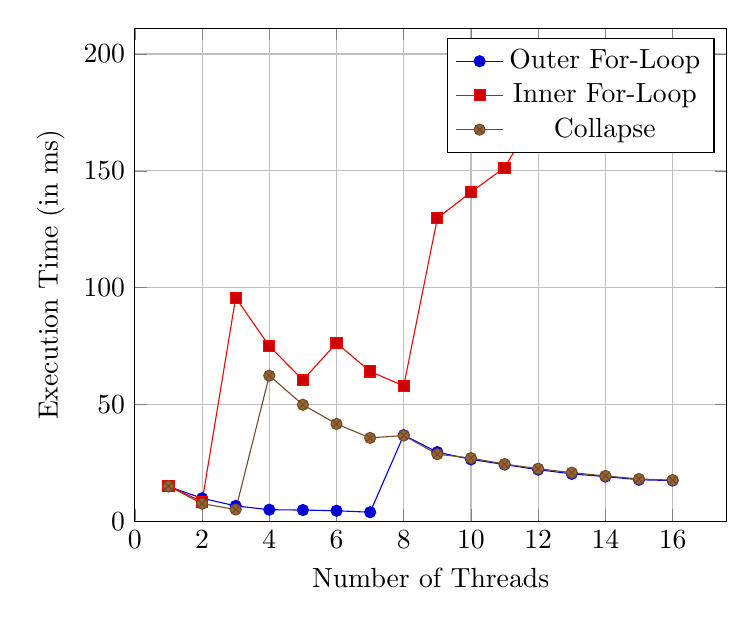
\begin{tikzpicture}
            \begin{axis}[
                title={},
                width=0.75\textwidth,
                xlabel={Number of Threads},
                ylabel={Execution Time (in ms)},
                xmin=0,
                ymin=0,
                grid=major
            ]
                \addplot coordinates {
                    (1,14.9234)(2,9.8524)(3,6.59485)(4,4.95885)(5,4.82065)(6,4.5133)(7,3.89165)(8,36.8866)(9,29.6062)(10,26.494)(11,24.2738)(12,22.0962)(13,20.3089)(14,19.1307)(15,17.7853)(16,17.4446)
                };
                \addlegendentry{Outer For-Loop}

                \addplot coordinates {
                    (1,15.243)(2,8.3793)(3,95.7094)(4,74.9772)(5,60.4569)(6,76.2988)(7,64.1251)(8,57.9691)(9,129.706)(10,140.856)(11,151.381)(12,175.358)(13,191.842)(14,171.761)(15,167.276)(16,189.499)
                };
                \addlegendentry{Inner For-Loop}       

                \addplot coordinates {
                    (1,15.0915)(2,7.557)(3,5.04065)(4,62.3426)(5,49.8704)(6,41.6652)(7,35.6859)(8,36.7201)(9,28.7093)(10,27.0565)(11,24.5003)(12,22.5038)(13,20.8165)(14,19.4369)(15,18.1129)(16,17.6074)
                };
                \addlegendentry{Collapse}
            \end{axis}
        \end{tikzpicture}
        \caption{Grayscale Performance Tests dice.png}
    \end{figure}
\end{center}